\documentclass[../uilmath.tex]{subfiles}
\graphicspath{{\subfix{../figures/}}}
\begin{document}
\chapter{Algebra}
\section*{Problems}
\begin{enumerate}[label=\bfseries\arabic*.]
    \item %% Problem 1 
    Evaluate: $1\times (2+3)^{-1}-4\div \frac{5}{6}+7\times(8)^0$
    
    \item %% Problem 2
    If $x$ is $40\%$ less than $y$ and $y$ is $30\%$ more than $z$, then $x$ is \blank than $z$.

    \item %% Problem 3
    Mora Doe goes to the 25\% off book sale. She buys 
    4 romantic novels which cost \$11.95 each before the sale 
    and includes tax. She gave the clerk 2 twenty-dollar bills. How much change should Mora receive?

    \item %% Problem 4
    If $9x^2-12x+4=(ax-b)^2$ then $a+b=\blank$.
    
    \item %% Problem 5
    Harry Hare drove 210 km to Myrtle Turtle's house. Part of the 4 hour trip was in town at 30 km/h 
    and the rest was on a major highway at 60 km/h. How many km did Harry drive on the major highway?

    \item %% Problem 6
    Simplify: $\log_b (3xy)-\log_b(\frac{3x}{2y})+\log_b (3y^2)$

    \item %% Problem 7
    Line $m$ goes through points $(1,-1)$ and $(-3,1)$. Line $n$ goes through points $(1,1)$ and $(x,y)$. Which of the following points lies on line $n$ if $m\perp n$?

    \item %% Problem 8
    Which of the equations will produce the shaded portion of the graph shown?
    \begin{center}
        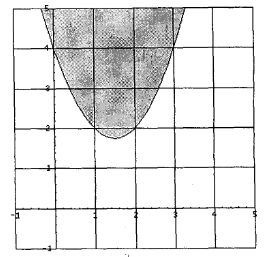
\includegraphics[width=0.3\textwidth]{2006SAC13.PNG}
    \end{center}

    \item %% Problem 9
    The first five terms of an infinite arithmetic sequence is $6\frac{1}{4},A,B,C,12\frac{1}{2},\dots$. Find $A+B+C$.

    \item %% Problem 10
    The numbers of integers that satisfy the inequality new $\frac{3}{7}<\frac{n}{14}<\frac{2}{3}$ is: 

    \item %% Problem 11 
    Define $n\star$ to be $n^n$. Compute $(2\star)\star$.

    \item %% Problem 12
    Evaluate: $\frac{3}{8}\div .75\times \frac{1}{2}-.25+\frac{1}{16}$

    \item %% Problem 13 
    A legend on a map shows 2.5 cm representing 200 miles. The distance on the map from El Paso to Texarkana is 9.8 cm. According to the map, how far is it from El Paso to Texarkana?

    \item %% Problem 14
    Phil Errup's car has a gas tank with a capacity of 18 gallons. The gauge shows that it is $\frac{1}{4}$ full. How many gallons will need to be added to the tank so that it is 75\% full?

    \item %% Problem 15
    Find the equation of the line shown.
    \begin{center}
        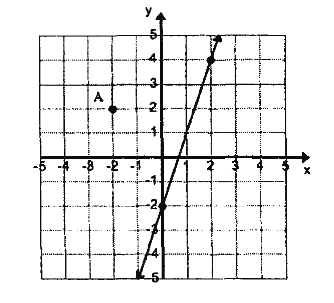
\includegraphics[width=0.3\textwidth]{2008SAC4.PNG}
    \end{center}

    \item %% Problem 16
    Let $p$ and $q$ be the roots of $8x^2+2x-15=0$. Find $p^3+3p^2q+3pq^2+q^3$.

    \item %% Problem 17
    One of the factors of $x^3-3x^2-3x+18$ is: 

    $\textbf{(A) } x+2 \qquad \textbf{(B) } x+3 \qquad \textbf{(C) } x+6 \qquad \textbf{(D) } x-2 \qquad \textbf{(E) } x-9$

    \item %% Problem 18
    The roots of the equation $x^3-5x^2+cx+24=0$ are $3,4$, and $R$. Find $c$.

    \item %% Problem 19
    Let $f(x)=2x+5$ and $g(x)=3x-4$ and $h(x)=6x$. Find $f(g(h(-1)))$.

    \item %% Problem 20
    The coefficient of the 2nd term of the expansion of $(3x-4)^5$ is: 

    \item %% Problem 21
    Solve for $k$ if $3k-4=28-5k$

    \item %% Problem 22
    Joe's dad sent him to the Burger Barn with three twenty-dollar bills and one five-dollar bill. He ordered 6 
    cheeseburgers for \$4.85 each, one basket of fries for \$5.75, 6 large cokes for \$2.19 each and 6 lemon pies for \$1.25 each.
    The tax rate is 8.25\%. How much change did he receive?

    \item %% Problem 23
    Consider a line that is perpendicular to $\overline{BC}$ and also contains point $A$. If the $x$-intercept of ths line is $(a,0)$, then $a=\blank$.
    \begin{center}
        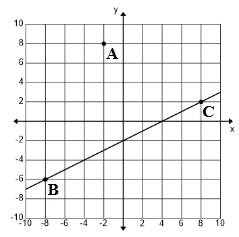
\includegraphics[width=0.3\textwidth]{2021SAC3.PNG}
    \end{center}

    \item %% Problem 24
    The Reagan High math/science team brought in the Quebe Sisters for a UIL fundraiser. Their fee to appear was \$5,000.
    Their version of ``San Antonio Rose'' is outstanding. A student ticket cost \$8.00 and an adult ticket cost \$15.00. A total of 
    2100 tickets were sold and \$20.375 was raised after paying the fee. How many adult tickets were sold?

    \item %% Problem 25
    Consider four consecutive even integers, all positive, such that five times the sum of the first two exceeds three times the sum of the first and fourth by 80. The third integer is \blank.

    \item %% Problem 26
    Simplify: $\frac{\frac{c}{w}+\frac{d}{w^2}}{\frac{m}{w^2}+\frac{k}{hw}}$

    \item %% Problem 27
    If $f(x)=x^2+4$ and $h(x)=3x-1$, then $f(h(5))=\blank$.

    \item %% Problem 28
    Find the number that is $\frac{5}{6}$ of the way from $-4\frac{1}{2}$ to $9\frac{3}{8}$.

    \item %% Problem 29
    Cindy rode her bike for 60 miles at 24 mph and then rode 36 miles at 30 mph. How fast does she need to ride 
    the final 44 miles to have an overall speed of 28 mph? (nearest tenth)

    \item %% Problem 30
    Consider the points $A(-6,10)$ and $B(4,-6)$. Find the equation of a line that exists such that every point on the line 
    is the same distance from $A$ as it is from $B$.

    \item %% Problem 31
    \begin{center}
        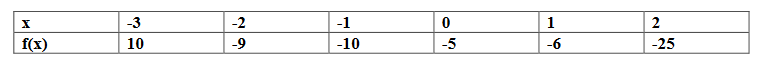
\includegraphics[width=0.7\textwidth]{2021SAC26.PNG}
    \end{center}

    Find the value of $f(-4)$.

    \item %% Problem 32
    If $s(x)$ is the slant asymptote of $h(x)=\frac{x^3+6}{2x^2+x-1}$, then $h(20)-s(20)=\blank$. (nearest thousandth)

    \item %% Problem 33
    If $(x^3-9x^2+kx-12)\div(x-1)$ has a remainder of zero, then $k=\blank$.

    \item %% Problem 34
    Consider the sequence $3,5,8,11,15,20,27,37,m,n,111,\dots$ $m+n=\blank$

    \item %% Problem 35
    Find the distance between the points $(3,5,7)$ and $(-4,1,-3)$. (nearest tenth)

    \item %% Problem 36
    Jeremy has 49 coins with a total value of \$7.05. He only has nickels, dimes, and quarters. He has three more quarters than nickels. How many dimes does he have?

    \item %% Problem 37
    Find the distance between point $A$ and the line shown on the right. (nearest tenth)
    \begin{center}
        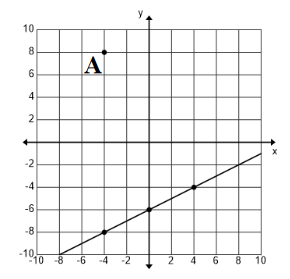
\includegraphics[width=0.3\textwidth]{2021SAC60.PNG}
    \end{center}

    \item %% Problem 38
    At Babe's in Sanger, we ordered four smoked chicken dinners for \$17.95 each, four iced teas for \$2.29 each and two 
    slices of apple pie for \$4.25 each. The tax rate was 8.125\% and I paid with one \$100 bill and one \$20 bill. I told the waitress to 
    keep the change as a tip. How much was her tip?

    \item %% Problem 39
    Consider the line with points $(-3,-5)$ and $(5,7)$. The line contains the point $(0,b)$. $b=\blank$.

    \item %% Problem 40
    Joe sets the motor of his small boat to travel at its maximum speed. At this setting, he travels 36 miles upstream, against the current, in 9 hours 
    and then turns around and travels 36 miles downstream, with the current, in 6 hours. What is the maximum speed of Joe's boat in still water?

    \item %% Problem 41
    Last summer, we drove from Lubbock, TX to McMinnville, OR to see relatives. On day 1, we drove 600 miles at an average speed of 
    62 mph. On day 2, we drove 620 miles at an average speed of 68 mph. On day 3, we drove 534 miles at an average speed of 60 mph. What was our overall average speed for the trip? (nearest tenth)

    \item %% Problem 42
    Jim can clean my pool in 75 min. Tom can clean my pool in 90 min. Julie can clean my pool in 60 min. If all three of them work together, how long would it take them to clean my pool? (nearest tenth)

    \item %% Problem 43
    Consider the line $y=f(x)$ which contains point $P$ and is parallel to the line shown below. Find the value of $f(9)$.

    \begin{center}
        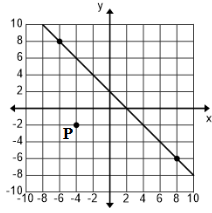
\includegraphics[width=0.3\textwidth]{2022SAC6.PNG}
    \end{center}

    \item %% Problem 44
    The UIL students at Latexo High School sold 246 tickets to the end of the year banquet. If adult tickets cost 
    \$18, student tickets cost \$12, and \$3816 was raised, how many student tickets were sold?

    \item %% Problem 45
    Mary has 57 coins that are either nickels, dimes or quarters. The value of the coins is \$8.60. She has ten more quarters than nickels. How many dimes does she have?

    \item %% Problem 46
    Find the number that is $\frac{3}{4}$ of the way from $-1\frac{1}{2}$ to $6\frac{5}{8}$.

    \item %% Problem 47
    If $f(x)=\frac{2x+5}{3-7x}$, then $f^{-1}(2)=\blank$.

    \item %% Problem 48
    Sixty workers could do 9 jobs in 6 days. How many days would it take 10 workers to do 12 jobs? (nearest tenth)

    \item %% Problem 49
    Consider the line $y=f(x)$ such that all points on the line are equidistant from the points $(-6,8)$ and $(4,-6)$. The $y$-intercept of the line $y=f(x)$ is $(0,b)$. $b=\blank$.

    \item %% Problem 50
    Find the domain of the function $f(x)=\frac{\sqrt{3+x}}{x^2-9x+20}$.

    \item %% Problem 51
    Solve the system 
    \begin{align*}
        \frac{2}{5}a+\frac{3}{10}c=2\frac{1}{5}\\
        -.5a+1.5b=2.5
        .75a-2.5c=-2
    \end{align*}
    $b=\blank$.

    \item %% Problem 52
    The points of intersection of the curves shown on the right are $P$ and $Q$. $PQ=\blank$. (nearest tenth)
    \begin{center}
        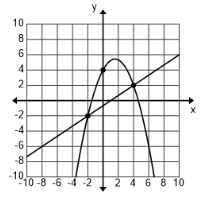
\includegraphics[width=0.3\textwidth]{2022SAC40.PNG}
    \end{center}

    \item %% Problem 53
    Joe and Arlene ate lunch at The Cotton Patch. Both ordered the Salmon Dinner which costs \$15.95 each and both 
    ordered peach iced tea which costs \$2.25 each. They shared a slice of chocolate cake which costs \$4.95. THe tax rate was 8.25\%.
    Joe was feeling generous so he paid with three \$20 bills and told the waitress to keep the change as a tip. How much was the tip?

    \item %% Problem 54
    An adult ticket to an Idaho Falls game cost \$10.00 and a youth ticket cost \$6.00. On Tuesday night's game, they sold 
    396 tickets and grossed \$3224. How many adult tickets did they sell?

    \item %% Problem 55
    Given: $f(x)=2x^2-6$ and $h(x)=e^x-8$. $f(h(3))=\blank$. (nearest hundredth)

    \item %% Problem 56
    Find the range of the function $f(x)=\frac{5}{\sqrt{x^2-1}}$.

    \item %% Problem 57
    Justin can wash and wax 10 cars in a 4 hours. Aryan can wash and wax 20 cars in 6 hours. Justin started work at 8:00 AM.
    Aryan arrived at 10:00 AM and they both worked from 10:00 AM until a total of 30 cars had been washed and waxed. What time was it when they finished 
    if they took no breaks? (nearest minute)

    \item %% Problem 58
    The roots of the quadratic equation $4x^2+bx+c=0$ are $-2.5$ and $1.5$. $b+c=\blank$.

    \item %% Problem 59
    The 5th term of an arithmetic sequence is 23 and the 13th term is 55. Find the sum of the first 15 terms of the sequence. 

    \item %% Problem 60
    Let $A = \begin{bmatrix}
        1  & -2\\
        1 & -3
        \end{bmatrix}$ and $B=\begin{bmatrix}
            -3 & 2\\
            -1 & 1 
        \end{bmatrix}$ and $AB = \begin{bmatrix}
            W & X \\
            Y & Z
        \end{bmatrix}$. What is the determinant of $AB$?

        \item %% Problem 61
        Which of the following is true about the relation $h(x)=5-x^2$?

        \item %% Problem 62
        Consider the sequence $17,21,25,29,33,37,\dots,129,133$. Find the sum of the terms of the sequence.

        \item %% Problem 63
        Eric is solving the equation $3x^2+3x-90=0$ by completing the square. On the third step, Eric adds \blank to both sides of the equation.

        \item %% Problem 64
        Consider the function $f(x)=4x^4-27x^3+cx^2+7x+30$. If $f(1)=14$, then $c=\blank$.

        \item %% Problem 65
        The graph of $f(x)=\frac{x^2-36}{x^3-x^2-30x}$ has $\blank$ asymptotes.

        \item %% Problem 66
        The sound level of a sound is given by $\beta = 10\log\left(\frac{I}{I_0}\right)$, where $\beta$ is the sound level in dB, $I$ is the intensity
        in W/m$^2$, and $I_0$ is the threshold of hearing which equals $10^{-12}$ W/m$^2$. Find the difference in sound levels for a sound with an 
        intensity of $7.75\times 10^{-3}$ W/m$^2$ and a sound with an intensity of $3.10\times 10^{-5}$ W/m$^2$. (nearest whole number)
        
        \item %% Problem 67
        The first three terms of an infinite geometric series are 84, 72, and 61$\frac{5}{7}$. Find the sum of the series.

        \item %% Problem 68
        Jack and Larry had supper at Bigham's Barbeque Friday night. Jack ordered the one-meat plate for \$16.75, a slice of chocolate cake for \$4.15, and an 
        iced tea for \$2.59. Larry ordered a two-meat plate for \$18.95 and an iced tea for \$2.59. The tax rate was 8.25\%. Jack was feeling generous so he paid with 
        three \$20 bills and told the waitress to keep the change as a tip. How much was the tip?

        \item %% Problem 69
        The Wylie math team held a fundraiser for their UIL team. They flew in the 60s rock group, the Ohio Express, and the concert was a sell-out.
        Adult tickets were priced at \$22.75 and student tickets were priced at \$14.50. They sold 2500 tickets and netted \$48,501.25. How many adult tickets did they sell?

        \item %% Problem 70
        If $f(x)=\sqrt{x^3+22}$ and $h(x)=\ln(x)+6$, then $f(h(55))=\blank$. (nearest tenth)

        \item %% Problem 71
        All of the houses on 6th street are the same size. Brennen can paint a house on 6th street by himself in 15 hours. If 
        Luke works with him, they can paint a house on 6th street in 8 hr 45 min. How long does it take Luke to paint a house on 6th street by himself? (nearest whole number)

        \item %% Problem 72
        The $y$-intercept of the line that contains the points $(-6,4)$ and $(12,-2)$ is the point $(0,b)$. $b=\blank$. (nearest tenth)

        \item %% Problem 73
        Find the domain of the function $f(x)=\frac{x-5}{\sqrt{9-x}}$.

        \item %% Problem 74
        The sound level of a sound is given by $\beta = 10\log\left(\frac{I}{I_0}\right)$, where $\beta$ is the sound level in dB,
        $I$ is the intensity in W/m$^2$, and $I_0$ is the threshold of hearing which equals $10^{-12}$ W/m$^2$. If the sound level is 
        98 dB, then the intensity is \blank W/m$^2$. (nearest ten-thousandth)

        
        For problems 75 and 76, consider a line containing points $A(-5,-1)$, $B(5,9)$, and $C(d,12)$.
        \item %% Problem 75
        The value of $d$ is \blank. (nearest tenth)

        \item %% Problem 76
        If the point $F(e,3)$ lies on the perpendicular bisector of $\overline{AB}$, then $e=\blank$.

        \item %% Problem 77
        Consider the function $f(x)=3x^3+bx^2-21x-30$. If $f(-2)=36$, then $b=\blank$.

        \item %% Problem 78
        The graph of $f(x)=\frac{x^2-16}{x^3+x^2-12x}$ has \blank asymptotes.

        \item %% Problem 79
        Consider the sequence $4,11,18,25,32,39,\dots$. Find the sum of the first 14 terms.

        \item %% Problem 80
        Consider the sequence $40,32,\frac{128}{5},\frac{512}{25},\dots$. Find the sum of the first 10 terms. (nearest tenth)

        \item %% Problem 81
        Evaluate $5!-5\times 5+5^5 \div 5$

        \item %% Problem 82
        Graphing calculators are on a ``buy 3 get 1 free'' special sale. The cost of a single calculator is \$85.50.
        Each calculator requires 4 batteries and a package of 6 batteries costs \$2.50 and are not sold by the individual battery.
        The tax rate is $8\frac{1}{2}$\%. What will the total cost be for 4 calculators, enough batteries to run them, and tax? (nearest cent)

        \item %% Problem 83
        The discriminant of $2x^2-3x+4=0$ is \blank. 

        \item %% Problem 84
        If $\frac{2y}{3}-\frac{3}{4x}=\frac{5y}{6}$, then $x$ equals \blank.

        \item %% Problem 85
        If $r$, $s$, and $t$ are real numbers such that $r+s+t=14$, $t^2=r^2+s^2$, and $rs=14$, find the value of $t$.

        \item %% Problem 86
        If $3^{x+y}=9$ and $4^{x-y}=64$ then $xy$ equals \blank.

        \item %% Problem 87
        Find $C$ if the remainder when $x^3-2x^2+x-5$ is divided by $x+C$ is 31.

        \item %% Problem 88
        In the expansion of $(3x-2y)^5$, the 4th term has a coefficient of \blank.

        \item %% Problem 89
        Simplify: $(\sqrt{x^{-20}y^{40}z^{-4}})^{\frac{1}{5}}$

        \item %% Problem 90
        An operation ``$\triangle$'' is defined by: $a\triangle b = a^b-b^a$. What is the value of 
        $(0\triangle 1)\triangle (1\triangle 2)$?

        \item %% Problem 91
        \begin{center}
            
\includegraphics[width=0.8\textwidth]{2006B27.PNG}
        \end{center}
        The distances between the hash marks ($\mid$) are equal. Find $S$.

        \item %% Problem 92
        30 miles per hour equals \blank feet per minute.

        \item %% Problem 93
        The function $f(x)=\mid 1-2x\mid-3$ crosses the $x$-axis at two points. Find the distance between the two points.

        \item %% Problem 94
        Dusty Rhodes flies from Durt E. Airport to Kleen X. Airport at a rate of 340 miles per hour. She rents a jeep
        and drives from Kleen X. Airport to Durt E. Airport at a rate of 60 miles per hour. How far is it from Kleen X. to Durt E.
        if the total traveling time was 2 hours and 30 minutes?

        \item %% Problem 95
        $x-1, 2x+3$ and $4x-5$ are factors of which of the following?

        $\textbf{(A) } 8x^3-10x^2-13x+15 \qquad \textbf{(B) } 8x^3-6x^2-17x+15 \qquad \textbf{(C) } 8x^3+6x^2-17x-15 \qquad \textbf{(D) } 8x^3-10x^2-17x+15 \qquad \textbf{(E) } 8x^3-6x^2-17x-15$

        \item %% Problem 96
        The point $P(-1,4)$ is rotated $90\degree$ clockwise around the origin to point $Q$. Then point $Q$ is reflected across the line 
        $y=x$ to point $R$. What are the coordinates of point $R$?

        \item %% Problem 97
        Mike Campbell is stacking soup cans at the Piggy Wiggy store for the weekend sale. The bottom row has 20 cans.
        Each successive row has 1 less can in it. If the top row has 3 cans, how many cans did Mike have on display?

        \item %% Problem 98
        If $a_1=1$, $a_2=3$, $a_3=4$ and $a_n = a_{n-1} + a_{n-2}$, where $n\geq 4$, then $a_9$ equals:

        \item %% Problem 99
        Which of the following is a false statement about the function $f$ whose graph is shown here?
        \begin{center}
            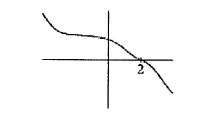
\includegraphics[width=0.3\textwidth]{2006B39.PNG}
        \end{center}

        \begin{align*}
            \textbf{(A)} \text{decreases monotonically} \qquad \textbf{(B)} \text{is positive at 0}\qquad \textbf{(C)} \text{has a zero at $x=2$} \\
            \textbf{(D)} \text{decreases monotonically in quadrant I} \qquad \textbf{(E)} \text{increases monotonically}
        \end{align*}


        \item %% Problem 100
        Let $f(x)=3x-2$ and $g(x)=2x+1$. Find the composite function $(g\circ f)(x)$.

        \item %% Problem 101
        General admission tickets at the ballpark cost \$3.00 for children under 12 and senior citizens over 55 and 
        \$5.00 for everyone else. On Tuesday, 2006 general admission tickets totaling \$8008.00 were sold. How many children
        and/or seniors bought general admission tickets?

        \item %% Problem 102
        Simplify: $\frac{(n+2)(n+1)!}{(n-1)(n-2)!}$

        \item %% Problem 103
        $P$, $Q$, and $R$ are the three real roots of $5x^3+4x^2-3x=2$. Find $PQ+QR+PR$.

        \item %% Problem 104
        The range of the function $y=\mid 1x-2 \mid +3$ is: 

        \item %% Problem 105
        Lotta Cash has a pocket full of change, but she can not make change for a dollar. Lotta has no half dollars 
        and no silver dollars. What is the greatest value of coins she could have?

        \item %% Problem 106
        Evaluate: $(3)^3\div (3+6)-3!\times \sqrt{9}$

        \item %% Problem 107
        70 miles per hour is equivalent to \blank inches per second.

        \item %% Problem 108
        Which of the following equations has a graph of a parabola that intersects the $y$-axis at only one point and the $x$-axis at only one point? $y=\blank$.
        
        $\textbf{(A) } .5x^2-2x+1 \qquad \textbf{(B) } x^2-4x-5 \qquad \textbf{(C) } |2x-4|+1 \qquad \textbf{(D) } 2\pm \sqrt{x} \qquad \textbf{(E) } 12(x)^{-1}$

        \item %% Problem 109
        Tryce Ikle can get to school in 12 minutes riding his bike at an average of 15 miles per hour (mph). How many minutes would it take him to walk to school if he walks at 4 mph?

        \item %% Problem 110
        If $x+y=5$ and $xy=1$ then $x^3+y^3=$?

        \item %% Problem 111
        Noah Sense is making a trapezoid using pennies. The bottom base is a row of 15 pennies. The next row above the base row 
        contains 1 less penny and each successive row contains 1 less penny. He continues until the top base of the trapezoid has only 3 pennies.
        How much money does he need to form the trapezoid of pennies?

        \item %% Problem 112
        The roots of the equation $x^3-bx^2+23x+d=0$ are $-1,9$, and $R$. Find $R$.

        \item %% Problem 113
        Let $A = \begin{bmatrix}
            2  & 3\\
            4 & x
            \end{bmatrix}$ and $B=\begin{bmatrix}
                y & 1\\
                -1 & -1 
            \end{bmatrix}$ then $AB = \begin{bmatrix}
                -1 & -1 \\
                1 & 1
            \end{bmatrix}$. Find $x+y$.

        \item %% Problem 114
        Two non negative numbers $x$ and $y$ exist such that the sum of the numbers is 12 and that the product of 
        one number and the square of the other number is a maximum. What is the maximum product?

        \item %% Problem 115
        Melody Toone's music store sells a new CD for 125\% above the wholesale cost. The store will buy the CD back in used 
        condition for 40\% of the selling price. How much profit will the store make if the selling price was \$19.99?

        \item %% Problem 116
        Which of the following system of inequalities would be best represented by the shaded region shown?
        \begin{center}
            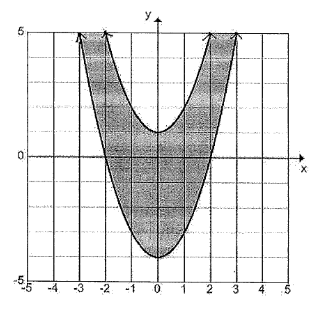
\includegraphics[width=0.3\textwidth]{2008B29.PNG}
        \end{center}

        \item %% Problem 117
        Mr. White and his dog walked 1 mile at an average speed of $3\frac{1}{3}$ mph and returned home the same route at an average speed of 
        $2\frac{1}{2}$ mph. What was their average speed for the entire walk?

        \item %% Problem 118
        The slope of the line tangent to the curve $y=x^3-5x+6$ at $x=1$ is $-2$. The point of intersection of the tangent line and the curve is:

        \item %% Problem 119
        Find the product of all the solutions of $16^{x^2+x+4}=32^{x^2+x}$.

        \item %% Problem 120
        The average of five tests is 85. If two test scores have 5 points removed from each, 1 test score has 20 points added, and the remaining two remain the same, the new average is:

        \item %% Problem 121
        Kandy Heart had a box of valentines. She gave $\frac{2}{3}$ of them to her classmates. She gave 5 of the remaining valentines to her brothers and sisters. SHe had 3 left over for her father, her mother, and herself.
        How many valentines were in the original box?
        
        \item %% Problem 122
        Line $6x-5y=4$ is perpendicular to line $3x-ay=1$. What is the value of $a$?

        \item %% Problem 123
        Line $AB$ is paralell to the line shown. Which of the following points could be point $B$?
        \begin{center}
            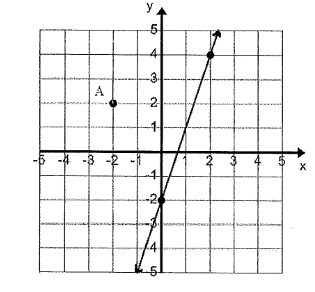
\includegraphics[width=0.3\textwidth]{2008B40.PNG}
        \end{center}

        $\textbf{(A) } (-7,-5) \qquad \textbf{(B) } (-6,-10) \qquad \textbf{(C) } (4,21) \qquad \textbf{(E) } (2,13) \qquad \textbf{(E) } (5,-1)$

        \item %% Problem 124
        The point $(3,4)$ is rotated 60 degrees clockwise about the origin. The coordinates of the point after the rotation is \blank. (closest approximation)

        \item %% Problem 125
        One of the roots of $ax^2+bx+c=0$ is $2-3i$. Find $b^2-4ac$, when $a=1$.

        \item %% Problem 126
        Evaluate: $(\log_2 8)(\log_3 9)(\log_4 4)$
    
        \item %% Problem 127
        How many asymptotes does this function have? $f(x)=\frac{x^2+6x+8}{x^2-6x+8}$.

        \item %% Problem 128
        Find the remainder when $f(x)=x^3+2x^2-3x-4$ is divided by $x-5$.

        \item %% Problem 129
        If $a_1=-3$, $a_2=1$ and $a_n=(a_{n-1})(a_{n-2})$, where $n\geq 3$, then $a_5$ equals:

        \item %% Problem 130
        Point $A(2,-4)$ lies in the $x-y$ plane. Point $A$ is reflected across the line $y=-x$ to point $B$. Point $B$ is reflected across the $x$-axis to point $C$.
        Point $C$ is reflected across the line $y=x$ to point $D$. Find the coordinates of point $D$.

        \item %% Problem 131
        The value of $(0.08333\dots)^{-1}\div (0.0625)^{-1}\times(.0555\dots)$ is:

        \item %% Problem 132
        Evaluate: $[1.2\div (\frac{3}{5})^2-(3)^{-1}]\times4!$

        \item %% Problem 133
        The distances between the hask marks (|) are equal. Find $P+R+S$.
        \begin{center}
            
\includegraphics[width=0.3\textwidth]{2009A2.PNG}
        \end{center}

        \item %% Problem 134
        Phil Upp's truck gets 17 miles per gallon of gas. He has \$20.00 to spend on gas. If the cost of a gallon of gas is \$3.50, how far can phil drive? (nearest whole mile)

        \item %% Problem 135
        Line $l$ going through points $(-1,3)$ and $(k,-5)$ is perpendicular to $x+4y=5$. Find $k$.

        \item %% Problem 136
        Simplify: $\left(\frac{6w^2+7w-3}{2w^3+5w^2+3w}\right)\left(\frac{w^2-w-2}{3w^2-7w+2}\right)$

        \item %% Problem 137
        Ima Whett paddles her kayak at a constant speed of 5 mph relative to the water. She paddles upstream for 
        1 hour 20 minutes. The return trip back only takes 1 hour 5 minutes. Which of the following is the closest approximation of the speed of the current?

        \item %% Problem 138
        The graph best depicts Mei Strol's daily 6 minute walk. (speed is not truly linear in this case). During the time interval of 3 minutes to 4 minutes Mei is \blank .

        \item %% Problem 139
        Let $x^5-x^4-px^3-qx^2-x-1=0$, where $p,q>0$. According to Descartes' Rule of Signs, how many possible roots are there?

        \item %% Problem 140
        If 5 adults and 2 teenagers work together, they can do a job in 1 day. If only 2 adults work, then 6 teenagers must 
        in order to do the job in 1 day. If no adults work and only 1 teenager works, how long will it take the teenager to do the job?

        \item %% Problem 141
        Missy Klas was absent the day of the algebra exam. She took the test the next day and made a 96. Her score raised the class average from 71 to 72.
        How many students, including Missy, took the test?

        \item %% Problem 142
        If the roots of $x^3+bx^2+cx+d=0$ are $-5,1$, and $3$, then $b+c+d$ equals:

        \item %% Problem 143
        Mr. White's college math class has 40 students. 75\% of the students are math majors. 32 of the students passed the final exam.
        75\% of those who passed the final exam are math majors. What percentage of the class who were not math majors passed the final exam?

        \item %% Problem 144
        If $y^2=-4+0i$ and $y^3=0-8i$ where $y=a+bi$ then $a+b$ equals:

        \item %% Problem 145
        How many of the following numbers are NOT solutions to $7-5|3x+1|\geq -1$?
        \begin{center}
            -0.987 \qquad -0.777$\dots$ \qquad .222$\cdots$ \qquad 0.3 \qquad .12
        \end{center}

        \item %% Problem 146
        Let $f(x)=4-x$ and $g(x)=3x-5$ and $h(x)=2x$. Find $h(f(g(0)))$.

        \item %% Problem 147
        How many asymptotes does $f(x)=\frac{2-3x^2}{x-1}$ have?

        \item %% Problem 148
        Evaluate: $2(3\times 4!\div (5-6)+7^2-8)$

        \item %% Problem 149
        What is 25\% of $\frac{3}{4}$ of 50 plus 75\% of $\frac{5}{8}$ of 40?

        \item %% Problem 150
        The Cheep Choppe is having a February Sale. The regular price of their special coats is \$89.95.
        They are on sale for 30\% off the regular price. A newspaper coupon offers 10\% off of the sale price. What would the selling price be if the customer brings in the coupon?

        \item %% Problem 151
        Find an equation of the line shown.
        \begin{center}
            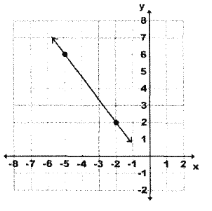
\includegraphics[width=0.3\textwidth]{2009B4.PNG}
        \end{center}

        \item %% Problem 152
        Betty Wheel rides her bicycle up and down the hilly streets from her house to school. The graph best depicts her 6 minute ride. (speed is not truly linear in this case).
        During the time interval of 2 minutes to 3 minutes Betty is \blank .
        \begin{center}
            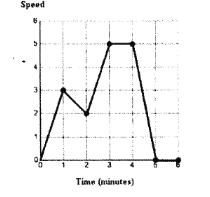
\includegraphics[width=0.3\textwidth]{2009B10.PNG}
        \end{center}

        \item %% Problem 153
        If 5 men working 5 hours a day for 5 days can dig a tunnel 5 km in length, then how long of a tunnel can 
        10 men working 10 hours a day for 10 days dig?

        \item %% Problem 154
        Lesleys Kwik runs the 400 meter dash at the local track meet. She runs the first 100 meters in 15 seconds, the second 100 meters in 16 seconds,
        the third 100 meters in 17.2 seconds and the last 100 meters in 18.5 seconds. What was her average speed? (nearest thousandth)

        \item %% Problem 155
        How many ordered pairs $(x,y)$ are solutions to the equation $5x+3y<40$, where $x,y$ are integers and $0<y<x<9$?

        \item %% Problem 156
        Find the smallest integer $k$ so that $4x^2=3x+k=0$ has two imaginary roots.

        \item %% Problem 157
        Let $f(x)=2x+1$ and $g(x)=4-3x$, then $f^{-1}[g^{-1}(-1)]$ equals:

        \item %% Problem 158
        If $p+q=12$ and $p\times q=22$ then $(p-q)^2=$?

        \item %% Problem 159
        Noah Kanwen won 40 of 75 games. How many of the next 25 games can Noah lose in order to have won 60\% overall?

        \item %% Problem 160
        Three students in Miss Woik's class were absent the day of the exam. The average of the other 12 students was 84.
        What would the three absent students have to average on their make-up exam in order to bring the entire class average to 86?

        \item %% Problem 161
        Find the determinant: 
        $A = \begin{bmatrix}
            -1 & 2 & 3\\
            1 & -2 & 3\\
            1 & 2 & -3
            \end{bmatrix}$
        
        \item %% Problem 162
        Simplify: $\frac{(n-1)!(n+2)!}{(n+1)!(n-2)!}$

        \item %% Problem 163
        Simplify: $((a^2b)^{-3}\times(ab^2)\div(a^2b^{-3})\times(ab))^{-1}$, where $a,b>0$.

        \item %% Problem 164
        In 3 years Sid Upp will be twice as old as his son, Stan Upp. Five years ago Stan's age was $\frac{1}{3}$ of his father's age at that time. What is the sum of their ages now?

        \item %% Problem 165
        Point $P(2,-3)$ is reflected across the origin to point $Q$. Then point $Q$ is translated horizontally 3 units to the right to point $R$.
        Point $R$ is reflected across the origin to point $S$. The coordinates of point $S$ is $(x,y)$. Find $x+y$.

        \item %% Problem 166
        If $9^{(x+2y)}=81$ and $9^{(2x-y)}=\frac{1}{9}$, then $3^{xy}=$?

        \item %% Problem 167
        Evaluate: $30-24\div 18\times 12+6$

        \item %% Problem 168
        Reid Moore went to the Ye Olde Book store to buy 3 copies of the same book for gifts. The regular price of the book is \$19.95.
        Because he is buying 3 copies, he gets 25\% off of the regular price of the second copy and 40\% off the regular price of the third copy.
        What would the total cost of the 3 books be before taxes? (to the nearest cent)

        \item %% Problem 169
        Using the partial ruler shown below, find the distance from $A$ to $B$.
        \begin{center}
            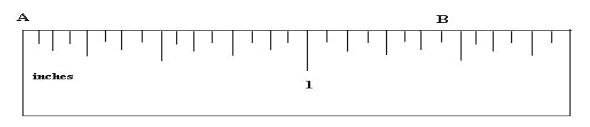
\includegraphics[width=0.3\textwidth]{2010A3.PNG}
        \end{center}

        \item %% Problem 170
        Which of the following is not a solution to $|8x-6|-4\geq 2$?

        $\textbf{(A) } -2\frac{1}{5} \qquad \textbf{(B) } -\frac{2}{5} \qquad \textbf{(C) } \frac{3}{5} \qquad \textbf{(D) } 1\frac{4}{5} \qquad \textbf{(E) } 2$

        \item %% Problem 171
        The function $f(x)=x^2-x-12$ crosses the $x$-axis at two points. Find the distance between the two points.

        \item %% Problem 172
        A male zebra fish has 8 stripes. A female zebra fish has 7 stripes. What is the ratio of male fish to female fish, if the 
        total number of stripes on all of the zebra fish in an aquarium totals 87?

        \item %% Problem 173
        Noah Sense has 28 coins consisting of pennies, nickels, and quarters. He has four times as many nickels as pennies and half as many quarters as nickels. How much money does he have?

        \item %% Problem 174
        If $8^{(k-1)}=16^{(3k)}$, then $4^{(k^{-1})}=$?

        \item %% Problem 175
        Find the determinant of the $2\times 2$ matrix 
        $A = \begin{bmatrix}
            -2 & 3\\
            5 & -7
            \end{bmatrix}$

        \item %% Problem 176
        Given the arithmetic sequence $15,a,b,c,47,\dots$, find $a+b+c$.

        \item %% Problem 177
        The number of integers that satisfy the inequality $\frac{4}{15}\leq \frac{n}{5} \leq 1\frac{1}{30}$ is: 

        \item %% Problem 178
        Simplify: $\frac{(n+1)!-(n-1)!}{(n-2)!}$

        \item %% Problem 179
        Simplify: $a^5 \div b^{-4} \times a^{-4} \times b^5 \div a^3 \times b^{-3}$

        \item %% Problem 180
        Simplify: $\frac{x^2-9}{4x+12}\div \frac{x^2-x-6}{x^2+2x}$

        \item %% Problem 181
        The distance from Abilene to Dallas by way of I30 is 185 miles. Ima Slow is leaving Abilene on I30 at 9:00 a.m. driving towards Dallas at 55 mph.
        Ura Quick is leaving Dallas on I30 at 9:00 a.m. driving toward Abilene at 70 mph. What time will they meet? (nearest minute)

        \item %% Problem 182
        If $a_1=2,a_2=4.5$, and $a_3=7$ are the first 3 terms of an arithmetic sequence, then $a_9=$?

        \item %% Problem 183
        The operation ``$\triangle$'' is defined by: $a\triangle b = a^b-b^a$. What is the value of $(0\triangle 1)\triangle(2\triangle 3)$?

        \item %% Problem 184
        Slim Sails rents kayaks and life vests for white water rafting. The kayak rental fee lats year was \$40 and the life vest rental fee last year was \$12.
        This year, the kayak rental fee increased 15\% and the life vest fee decreased 25\%. What is the overall percent increase in rental fees for the kayak and vest 
        from last year to this year? (nearest tenth)

        \item %% Problem 185
        If $-3(2-x)=2(x+3)$ then $(2x-3)$ equals:

        \item %% Problem 186
        Find the slope of a line perpendicular to the line drawn in the graph below.
        \begin{center}
            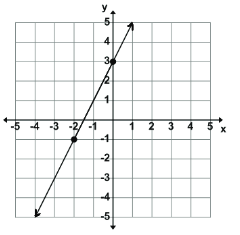
\includegraphics[width=0.3\textwidth]{2010A51.PNG}
        \end{center}

        \item %% Problem 187
        Let $f(x)=2-5x$ and $g(x)=3x+5$. If $h(x)$ is the inverse function of $\frac{f(x)}{g(x)}$, then $h(-4)=$?

        \item %% Problem 188
        The polynomial $2x^4-8x^2+x+5$ has at most \blank negative zeros.

        \item %% Problem 189
        Evaluate: $\frac{7}{8}+\frac{3}{4}\div(\frac{5}{8}-\frac{1}{2})\times \frac{3}{8}+\frac{1}{4}-\frac{1}{8}$

        \item %% Problem 190
        Using the partial ruler shown below, find the distance from $A$ to $B$.
        \begin{center}
            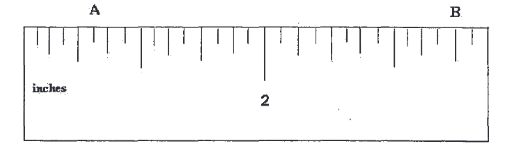
\includegraphics[width=0.3\textwidth]{2010B2.PNG}
        \end{center}

        \item %% Problem 191
        May B. Fishy has a salt water aquarium. She mixes 5 gallons of water with some salt to make a 20\% saline solution.
        The fish require a 16\% solution. How much water will she have to add to make the required 16\% saline solution?

        \item %% Problem 192
        Find $f(5)+f(-1)+f(2)$ if 
        $f(x)=\begin{cases}
            x - 3 & \text{if } x<0\\
            3x & \text{if } 0<x<3 \\
            3-x  & \text{if } x>3
        \end{cases}$

        \item %% Problem 193
        If $y=1-x$ and $y=\frac{2}{x}$ then $(x+y)(x^2-xy+y^2)=$?

        \item %% Problem 194
        Find the quotient: $(x^4+2x^3-10x^2+22x-15)\div (x^2-2x+3)$

        \item %% Problem 195
        Les Moolah has 28 coins. The coins are nickels and quarters and have a total value of \$4.00. How many more nickels than quarters does Les have?

        \item %% Problem 196
        Find $k$ if $x+4$ is a factor of $x^3-x^2+kx+12$.

        \item %% Problem 197
        On the map legend, 1 inch represents 120 miles. Beautiful downtown Millersview is 45 miles from San Angelo. How far is it on the map?

        \item %% Problem 198
        Which of the following is not a solution of $3+2|5x-1|\leq 4$?

        $\textbf{(A) } \frac{1}{4} \qquad \textbf{(B) } \frac{2}{5} \qquad \textbf{(C) } \frac{1}{6} \qquad \textbf{(D) } \frac{2}{7} \qquad \textbf{(E) }\frac{1}{8}$

        \item %% Problem 199
        Which of the equations will produce the shaded portion of the graph shown?
        \begin{center}
            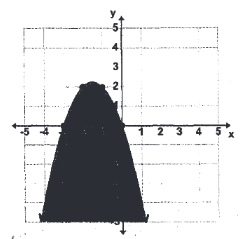
\includegraphics[width=0.3\textwidth]{2010B28.PNG}
        \end{center}

        \item %% Problem 200
        The Azusa Aztec band is selling band calendars to make money for their trip. They get 30\% of the sales for the first 100 sold,
        40\% of the sales above 100 but less than or equal to 200, and 50\% of the sales over 200. How much will the band make if they sell 275 calendars if each calendar sells for \$10.

        \item %% Problem 201
        Simplify: $a^{-2}\times b^2 \div a^3\div b^{-3}\times a\div b$

        \item %% Problem 202
        The points $(2,3)$ and $(-4,k)$ lie on the line $5x-6y=C$. Find $k$.

        \item %% Problem 203
        Les Quik, Moe Fass, and Willie Makit run in a 100 meter race. Les beat Moe by 10 meters and Moe beat Willie by 20 meters.
        If the runners ran at a constant speed, by how much did Les beat Willie?

        \item %% Problem 204
        Point $P(-3,2)$ and point $Q(4,-5)$ line on the $x-y$ plane. $P$ is translated horizontally 2 units to the left. $Q$ is reflected 
        across the $y$-axis. What is the distance between the points after the translations? (nearest tenth of a unit)

        \item %% Problem 205
        If $a_1=2$, $a_2=3$, $a_3=5$ and $a_n=a_{n-1}+a_{n-2}-a_{n-3}$, where $n\geq 4$, then $a_8$ equals:

        \item %% Problem 206
        Find $f(g(1-x))$ when $f(x)=3x-1$ and $g(x)=x-3$.

        \item %% Problem 207
        Find an equation of a line parallel to line $AB$ and passing through point $(-2,-3)$.
        \begin{center}
            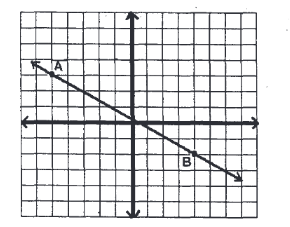
\includegraphics[width=0.3\textwidth]{2010B45.PNG}
        \end{center}

        \item %% Problem 208
        Find the determinant of the $3\times 3$ matrix.
        $\begin{bmatrix}
            1 & 1 & 2 \\
            2 & 1 & 3 \\
            -1 & 0 & 1
        \end{bmatrix}$

        \item %% Problem 209
        $R_1, R_2$ and $R_3$ are the roots of the equations $24x^3+26x^2-19x-6=0$. $R_1$ and $R_2$ are the roots of the equation 
        $12x^2-5x-2=0$ as well. Find $R_3$.

        \item %% Problem 210
        Let $x=\frac{1}{2+\frac{1}{3+\frac{1}{2+\frac{1}{3+\dots}}}}$ be the continued fraction. Find $x$.

        \item %% Problem 211
        Simplify: $\frac{(n+1)!}{(n-1)!}\div \frac{(n+2)!}{n!}$

        \item %% Problem 212
        Evaluate: $4!\times (4)^{-2}+(4^2)^{\frac{1}{4}}-4\div 2$

        \item %% Problem 213
        Lotta Cash received a \$50.00 gift card for graduation. She went shopping at the Cheap Shoppe. She bought 2 pairs of shorts at \$7.99 each, 3 pair of flip-flop 
        sandals at \$4.50 each, a bottle of suntan lotion at \$8.25, a sun hat at \$9.89, and 2 bottles of water at 75\textcent  each. She got 15\% off for using a gift card 
        instead of a credit card. How much does she have left on her gift card if the tax rate was 7.5\%.
        
        \item %% Problem 214
        If $45\%$ of $A$ is $4\frac{1}{5}$ of $B$, then $B$ is what percent of $A$?

        \item %% Problem 215
        Which of the inequalities is best represented by the graph below?
        \begin{center}
            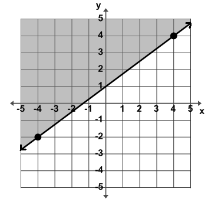
\includegraphics[width=0.3\textwidth]{2018A5.PNG}
        \end{center}

        \item %% Problem 216
        Simplify: $\left(\frac{2x^2-7x+5}{4x^2+8x-12}\right)\div \left(\frac{4x^2-8x-5}{2x^2+73}\right)$

        \item %% Problem 217
        If $4x^2-x+c = (ax+b)(x+1)$ then $a+b+c=$\blank .

        \item %% Problem 218
        The line $y=mx+b$ contains the point $(-5,-2)$ and has a slope of $-\frac{3}{4}$. The $y$-intercept is:

        \item %% Problem 219
        A rectangular swimming pool is twice as long as it is wide and has a 10 foot-wide concrete border around it.
        If the border has an area of 2800 sq. ft., find the perimeter of the pool.

        \item %% Problem 220
        If $27^{(k)}=9^{(k+1)}$, then $3^{(k+2)}=$?

        \item %% Problem 221
        Let $f(x)=x-2$, $g(x)=2x-1$, $h(x)=3x$, and $g(f(x))+f(h(x))=-4$. Find $x$.

        \item %% Problem 222
        Which of the following does not have an inverse function?

        $\textbf{(A) } y=2x-4 \qquad \textbf{(B) } y=\frac{1}{4}x+2 \qquad \textbf{(C) } y=-x^2+4 \qquad \textbf{(D) } y=\ln(x+4) \qquad \textbf{(E) }y=\sqrt{2x-4}$

        \item %% Problem 223
        Phil Dewallit got a \$20.00 allowance for mowing his parent's lawn this week. They agreed to increase his previous week's allowance 
        80\textcent  each week for the next 24 weeks. Phil decides to put half of his allowance in his piggy bank each week.
        How much will he have in the bank at the end of the 25 week period?

        \item %% Problem 224
        In the expansion of $(3x-2)^5$, the sum of the coefficients of the 3rd and the 4th term is:

        \item %% Problem 225
        $\sum_{k+1}^3 (-1)^k(kx-(k+1)y-k)=$?

        \item %% Problem 226
        Sameer, Anisha, and Ian worked a total of 125 problems on the number sense test at the math camp.
        Sameer worked 28\% of the total problems, Anisha worked 40 less problems than Ian did. What percent of problems did Ian work?

        \item %% Problem 227
        Find $a+b+c+d$ given the arithmetic sequence: $-11, a,b,c,3,d,\dots$

        \item %% Problem 228
        Let $f(x)=ax^3-bx+3$ where $a$ and $b$ are integers. If $f(2)=-4$, then $f(-2)=$?

        \item %% Problem 229
        Coach Ball has 22 students in his PE class. 9 of the students play football, 10 play basketball, 5 play tennis and basketball but not football,
        5 play basketball and football but not tennis, and 2 play tennis only. How many students do not play any of these 3 sports?

        \item %% Problem 230
        I. Cee and U. Saul used a 2 in. $\times$ 12 in. $\times$ 16 ft. board to make a teeter-totter with the center being on a fulcrum.
        Cee weighs 85 pounds and is sitting 8 feet from the center of the teeter-totter. Saul weighs 100 pounds and is sitting on the opposite end.
        How far from the center should Saul sit if the teeter-totter has a slope of zero? (nearest inch)

        \item %% Problem 231
        If $\log_6(16)-\log_6(4x)=\log_6(x+2)$, then $x$ equals \blank .

        \item %% Problem 232
        Let $g(x)=3x^2-2x+1$. Find $k$ is $g(k-1)-g(k)=11$.

        \item %% Problem 233
        How many ordered pairs of positive integers $(a,b)$ with $a+b\leq 50$, satisfy the equation: $(a+b^{-1})\div (a^{-1}+b)=13$.

        \item %% 234
        If $x<y$ and $x<0$, which of the following is never greater than any of the others?

        $\textbf{(A) } x+y \qquad \textbf{(B) } x-y \qquad \textbf{(C) } x+|y| \qquad \textbf{(D) } x-|y| \qquad \textbf{(E) } -|x+y|$

        \item %% 235
        Given the sequence, $\frac{7}{(1\times 1+1)}-\frac{7}{(2\times 2-1)}+\frac{7}{(3\times 3+1)}-\frac{7}{(5\times 5-1)}+\frac{7}{(8\times 8+1)}-\dots$, find the digit 
        in the ten-thousandths place. 

        \item %% 236
        Evaluate: $\sqrt[3]{1728}\div (16)^{\frac{1}{2}}+8\times (2)^{-1}-4$

        \item %% 237
        Two and one-fourth million is added to three hundred twenty thousand five hundred. One million one thousand one hundred is subtracted from the sum. The difference is divided by 
        eleven. The quotient is truncated to the units place. Which digit appears the most in the final results?

        \item %% 238
        If $(3x+1)(x-3)(2x)=ax^3+bx^2+cx+d$ then $a+b+c+d=$ \blank . 

        \item %% 239
        A line parallel to the line shown through the point $(1,-1)$ has $x$-intercept at point $(a,b)$ and $y$-intercept at point $(c,d)$. Find $a+b+c+d$.
        \begin{center}
            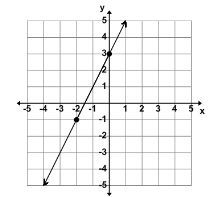
\includegraphics[width=0.3\textwidth]{2018B6.PNG}
        \end{center}

        \item % 240
        Max Whale likes to mix his regular blend coffee with a boost blend coffee at a ratio of 3 to 1. The regular blend sells for \$11.00 per pound and the boost blend sells for \$8.00 per pound.
        Find the cost per pound of Max's special mixture of regular blend and boost blend. (nearest cent)

        \item % 241
        What is the only real number which, when divided by itself, is 2020 times itself?

        \item % 242
        What is the smallest perfect square that can be written as the sum of three different prime numbers?

        \item % 243
        Gerry arrived at the bus stop $x$ hours past noon. Dale arrived 4 hours later. Pat arrived at 5 P.M., $x$ hours after Dale. At which time did 
        Gerry arrive at the bus stop? 

        \item % 244
        For what value of $x>0$ does $\frac{x^2+2021x+2020}{x^2-2020x-2021}=2$?

        \item % 245
        What is the greatest integer that always divides the difference of the squares of any two different positive odd integers?

        \item % 246
        Of the positive integers between 1000 and 10000 that are divisible by 8, how many have a hundreds digit of 5?

        \item % 247
        Les Square increased the length of two opposite sides of a square by 20\%, and decreased the other two opposite sides by 50\%. What percent of the area of the original square is the area of the new rectangle?

        \item % 248
        If $\frac{x+5}{2x-1}+\frac{Ax+B}{3x+2}=\frac{-7x^2+30x+6}{6x^2+x-2}$, where $A$ and $B$ are constants, then $A+B$ equals:

        \item % 249
        Let $f(x)=2x-1$ and $g(x)=2-3x$ and $h(x)=x+3$. Find $g(h(f(1-x)))$.

        \item % 250
        The graph of $f(x)=Ax^3+Bx^2+Cx+D$ is shown here. Find $A+B+C+D$.
        \begin{center}
            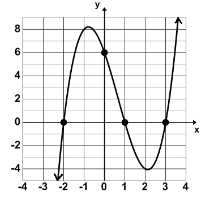
\includegraphics[width=0.3\textwidth]{2018B14.PNG}
        \end{center}

        \item % 251
        Les Qwik and Lotta Speed worked together to finish their research project in 12.5 hours. Lotta works 
        2.5 times faster than Les. How long would it have taken Lotta to do the project alone?

        \item %252
        How many negative real roots will $x^5+x^4-2x^3+x^2-1=0$ have?

        \item %253
        Which of the following is true about the function $f(x)=\frac{x^2+4}{x^3-3}$?

        I. $f(x)$ is odd \qquad II. $f(x)$ is even \qquad III. $f(x)$ has 3 asymptotes.

        \item % 254
        Find $k$ if $GCF(48,k)=8$ and $LCM(48,k)=336$.

        \item % 255
        $\{(x,y)|x,y \in {\text{Integers}}, -10\leq x\leq 10, \text{and } -10\leq y\leq 10\}$ is the solution set of $2x+5y=10$. How many such ordered pairs exist?

        \item % 256
        Find $C$ if the remainder when $(3x^3+2x^2-x+C)\div (x+1)$ is $4$.

        \item % 257
        Ester Bunnee had a box of chocolate eggs. She hid half of them in the yard for the big hunt.
        Then she put two of the remaining eggs in her room for a late night snack. The remaining six eggs were put in the refrigerator 
        for a later day. How many chocolate eggs were in the original box?

        \item % 258
        If $12x^2+ax-5=(bx-5)(2x+c)$ then $abc=\blank$.

        \item % 259
        Let $e^{(2x-3)}=4e^{5x+6}$. Find $e^{(x)}$. (nearest hundredth)

        \item % 260
        Let $f(x)=ax+4$ and $g(x)=bx-1$, where $a$ and $b$ are positive integers. Find $a+b$ if 
        $f(g(x))=g(f(x))$.

        \item % 261
        In honor of Valentines day, let $x=2+\frac{14}{2+\frac{14}{2+\frac{14}{2+\frac{14}{2+\dots}}}}$. Find $x$. (nearest tenth)

        \item % 262
        The fraction $\frac{30}{\sqrt{3}+\sqrt{5}+\sqrt{8}}$ can be written as $a\sqrt{30}+b\sqrt{3}+c\sqrt{5}+d\sqrt{8}$. Find $a+b+c+d$.

        \item % 263
        Let $f(x)=\sqrt{6-\sqrt{2x+7}}$. The domain of $f(x)$ is ${x|p\leq x\leq q}$. Find $\frac{P+Q}{2}$.

        \item % 264
        Given: $9x-6y=21$ and $6x-4y=k$. Find the value of $k$ such that the system of equations has an infinite number of solutions.

        \item % 265
        Evaluate $[4!-(3)^3]+2^{-2}\times \sqrt{2^4\div 3^4}$

        \item % 266
        Will Itkosmoor wants to buy 4 new calculators for his math team. He can buy 2 at the regular price, 2 at the half price, and pay 
        8\% of the total price for shipping and handling. He can get 16\% off and pay no shipping if he buys 4 at the regular price.
        If the regular price is \$89.95, how much will he save if he takes the best deal? (tax exempt)

        \item % 267
        Evaluate: $1+11^2\div (2+9)+1\times 9$

        \item % 268
        Mae B. Tulong had twelve yards of rope. She cut off a length of rope that was 2 yards 1 foot 8 inches long.
        Then she divided the remaining length of rope into four equal parts. How long was each of the four equal parts of rope?

        \item % 269
        Which of the following points lies on a line parallel to the line shown and containing point $(0,3)$?
        \begin{center}
            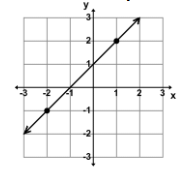
\includegraphics[width=0.3\textwidth]{2019A5.PNG}
        \end{center}

        $\textbf{(A) } (9,6) \qquad \textbf{(B) } (7,11) \qquad \textbf{(C) } (11,15)\qquad \textbf{(D) }(-7,-4) \qquad \textbf{(E) } (-12,-12)$

        \item % 270
        Let $4x^2+17x-15=(ax+b)(cx+d)$. Find $a+b+c+d$.

        \item % 271
        Let $(2x-1)^2(2x+1)=ax^3+bx^2+cx+d$. Find $a+b+c+d$.

        \item % 272
        Simplify: $\left(\frac{x^2-3x-10}{x^2+2x-35}\right)\div \left(\frac{x^2+9x+14}{x^2+4x-21}\right)$

        \item % 273
        If $\frac{3x+2}{x-1}-\frac{x-3}{2x+1}=\frac{ax^2+bx+c}{dx^2+ex+f}$, then $a+b+c+d+e+f$ equals:

        \item % 274
        If $a_1=1, a_2=3, a_3=-5$ and $a_n=a_{n-1}+a_{n-3}-a_{n-2}$, where $n\geq 4$, then $a_6$ equals:

        \item % 275
        Let $x-3y=5$ and $2y+z=3$ and $2-z=x$. Find $x+yz$.

        \item % 276
        If $f(x)=x^2-3x+2$ and $g(x)=2x^2-x+3$, then $g(f(4))=$?

        \item % 277
        $(8x^3-4x^2-2x+1)\div (2x+1)$ has a remainder of \blank .

        \item % 278
        Find the absolute value difference between coefficients of the $x^2y^3$ term and the $x^3y^2$ term in the expansion of $(3x+2y)^5$.

        \item % 279
        Find the 20th term of the sequence: $3,8,15,24,35,48,\dots$

        \item % 280
        The Shawk Electric Company charges a monthly base fee of \$10.50 and a usage fee of 8\textcent per kilowatt hour used.
        The company offers a \$25.00 credit if the kilowatt usage is over 1200 kWh. How much would the bill be before taxes if the monthly usage was 1450 kWh.

        \item % 281
        Two billion three hundred four million five thousand sixty-seven is added to twenty-three million four hundred fifty-two thousand 
        six hundred seven. Which of the following digits appears the most in the sum?

        \item % 282
        Soh Yung is 3 times as old as her sister Tu Yung. In 4 years Soh will only be twice as old as Tu. What will the sum of their ages be in 10 years?

        \item % 283
        PurtyDurty detergent contains 80\% soap and 20\% bleach. WishyWashy detergent contains 55\% soap and 45\% bleach.
        If PurtyDurty is mixed with WishyWashy, what percent of the mixture should be PurtyDurty if the final mixture is 35\% bleach?

        \item % 284
        Let $P$ and $Q$ be the roots of $4x^2+17x=15$. Find $(P+Q)(PQ)$.

        \item % 285
        Let $\begin{bmatrix}
            -1 & -2 \\
            1 & 3
        \end{bmatrix}\times \begin{bmatrix}
            2 & 1 \\
            -3 & -4
        \end{bmatrix}=
        \begin{bmatrix}
            a & c \\
            b & d
        \end{bmatrix}$. Find $a+b+c+d$.

        \item % 286
        Let $f(x)=ax^2+bx+5$ where $a$ and $b$ are integers. If $f(1)=2$ and $f(2)=3$, then $f(3)=$?

        \item % 287
        8,051 is the product of the two prime factors. The sum of these two prime factors is?

        \item % 288
        Which of the following is/are not function(s)?

        $\textbf{I. } \{(2,6),(-3,6),(4,9),(2,10)\}$

        $\textbf{II. } \{(1,3),(2,3),(3,3),(4,3)\}$

        $\textbf{III. } \{(-2,2),(-1,1),(0,0),(1,1)\}$

        \item % 289
        Which of the following points does not lie on the line containing the point $(-2,-3)$ and having a slope of $-1.5$?

        $\textbf{(A) } (-5,1.5) \qquad \textbf{(B) } (-8,6) \qquad \textbf{(C) } (7,-15.5) \qquad \textbf{(D) }(4,-12) \qquad \textbf{(E) } (9,-19.5)$

        \item % 290
        Let function $f$ be defined as $f(x)=2x-6$ for all real numbers.

        Let function $g$ be defined as follows for all integers that $-3\leq x\leq 3$:
        \begin{center}
            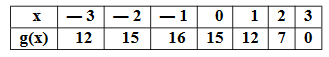
\includegraphics[width=0.3\textwidth]{2019A58.PNG}
        \end{center}

        Which of the following is true about both functions $f$ and $g$?

        \textbf{(A) } They reach their maximum value at the same domain value \\
        \textbf{(B) } They have the same $y$-intercept \qquad \textbf{(C) } They are both odd functions \\
        \textbf{(D) } They share an $x$-intercept \qquad \textbf{(E) } none of these are true 

        \item % 291
        After math practice on Thursday, the Holliday math team drove to the Whataburger in Wichita Falls for supper. The principal 
        gave them \$50 to spend. They ordered 5 cheeseburger combos. A combo cost \$7.85 plus tax. If the tax rate is 8.25\% and if an apple pie cost 
        \$1.25 plus tax, how many apple pies could they order?

        \item % 292
        To pay for some new HP Prime G2 calculators for Mr. C's math team, Crosby, Stills, and Nash agreed to perform at SHS with all proceeds going to the math 
        department. Student tickets cost \$15.00 and adult tickets cost \$25.00. If they raised \$7,700 by selling 
        372 tickets, how many adult tickets were sold?

        \item % 293
        Line $L_1$ contains the points $(-8,6)$ and $(4,-10)$. Line $L_2$ is parallel to $L_1$ and contains the point $(-6,-12)$. The $y$-intercept of $L_2$ is $(0,b)$. The value of $b$ is \blank .

        \item % 294
        Tal rented a car at the airport where his plane landed in Boise. The city of Boise charges an upfront fee of \$20 to rent a car at the airport. He was also 
        charged \$25 per day and \$0.55 per mile. If Tal used his car for five days and his final bill was \$241.25, how many miles did he drive during his stay?

        \item % 295
        Anthony can wash and wax a car in 45 minutes while Jacob needs one hour to wash and wax a car. If Anthony works by himself for two hours before 
        being joined by Jacob, how much time will it take for them to wash and wax 16 cars? (nearest minute)

        \item % 296
        The value of Warith's house is increased by 9.35 percent each year. If his house is worth \$378,000 on January 1st, 2023, 
        what should it be worth on January 1st, 2035? (nearest dollar)

        \item % 297
        If the values of the roots of the function $f(x)=7x^2+14x-105$ are $a$ and $b$, then $\frac{a+b}{ab}=\blank$.


        Use the following graph for problems 298 and 299.
        \begin{center}
            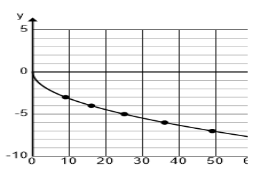
\includegraphics[width=0.3\textwidth]{uil2023district8.PNG}
        \end{center}
        \item % 298
        The graph of $y=h(x)$ begins at the point $(0,0)$. $h(121)=\blank$.

        \item % 299
        If $g(x)$ is the inverse function of $h(x)$, find the domain of $g(x)$.

        \item % 300
        The number of 2-liter cokes sold at Walmart each month varies inversely as the price. In a month when the price was 
        \$1.80, they sold 3448 2-liter cokes. If the price is reduced to \$1.20 the next month, what is the expected number of cokes that will be sold?

        \item % 301
        Consider $f(x)=2x^3+bx^2+4x-8$. If $f(3)=31$, then $b=\blank$.

        \item % 302
        Consider four consecutive even negative integers (in increasing order) such that the product of the first and third 
        is 122 greater than the product of $-25$ and the fourth. Find the sum of the four integers.

        \item % 303
        Consider an arithmetic sequence in which the sixth term is 47 and the twelth term is 95. What is the product of the eighteenth and nineteenth terms?

        \item % 304
        If $f(x)=\frac{3x-4}{5x-6}$ and $h(x)=\frac{-2x+5}{-3x-8}$, then $\left(h^{-1}\circ f^{-1}\right)(1)=$

        \item % 305
        Three of the roots of the fourth-degree polynomial $x^4+bx^3+cx^2+dx+e$ are $-2,3$, and $1-\sqrt{5}$. If $b$, $c$, $d$, and $e$
        are rational numbers, then $b+c+d+e=\blank$.

        \item % 306
        The sound level in decibels, $\beta$ is given by $\beta = 10\log\left(\frac{I}{10^{-12}}\right)$, where $I$ is the intensity of sound in W/m$^2$.
        Andrew is playing his trumpet, producting a sound level of 88 dB. If twelve other musicians join him and they all play their trumpets at the same intensity as Andrew,
        what is the sound level of all of the trumpets playing together? (nearest whole number)

        \item % 307
        
\end{enumerate}

\section*{Solutions}
\begin{enumerate}[label=\bfseries\arabic*.]
    \item %% Problem 1
    $2 \frac{2}{5}$

    \item %% Problem 2
    22\% less

    \item %% Problem 3
    \$4.15 

    \item %% Problem 4
    5

    \item %% Problem 5
    180 km

    \item %% Problem 6
    $4\log_b (6y)$

    \item %% Problem 7
    $(-1,-3)$

    \item %% Problem 8
    $y>x^2-3x+4$

    \item %% Problem 9
    $28 \frac{1}{8}$

    \item %% Problem 10
    3

    \item %% Problem 11
    256 

    \item %% Problem 12
    .0625 

    \item %% Problem 13 
    784 miles 

    \item %% Problem 14
    9 

    \item %% Problem 15
    $3x-y=2$

    \item %% Problem 16
    $-\frac{1}{64}$

    \item %% Problem 17 
    A 

    \item %% Problem 18
    -2 

    \item %% Problem 19
    -39 

    \item %% Problem 20
    -1620 

    \item %% Problem 21
    4

    \item %% Problem 22
    \$4.93 

    \item %% Problem 23
    2.0 

    \item %% Problem 24
    1225 

    \item %% Problem 25
    26

    \item %% Problem 26
    $\frac{chw+dh}{hm+kw}$

    \item %% Problem 27
    200

    \item %% Problem 28
    $7\frac{1}{16}$

    \item %% Problem 29
    33.8 mph

    \item %% Problem 30
    $5x-8y=-21$

    \item %% Problem 31
    55

    \item %% Problem 32
    0.025 

    \item %% Problem 33
    20

    \item %% Problem 34
    127

    \item %% Problem 35
    12.8

    \item %% Problem 36
    12

    \item %% Problem 37
    14.3

    \item %% Problem 38
    \$23.27

    \item %% Problem 39
    -0.50 

    \item %% Problem 40
    5.0 mph

    \item %% Problem 41
    63.3 mph 

    \item %% Problem 42
    24.3 min 

    \item %% Problem 43
    -15 

    \item %% Problem 44
    102 

    \item %% Problem 45
    19

    \item %% Problem 46
    $4\frac{19}{32}$

    \item %% Problem 47
    $\frac{1}{16}$

    \item %% Problem 48
    48.0 days 

    \item %% Problem 49
    $\frac{12}{7}$

    \item %% Problem 50
    $x\geq -3, x\neq 4,5$

    \item %% Problem 51
    3

    \item %% Problem 52
    7.2 

    \item %% Problem 53
    \$15.24

    \item %% Problem 54
    212

    \item %% Problem 55
    286.12

    \item %% Problem 56
    $(0,\infty)$

    \item %% Problem 57
    2:17 PM 

    \item %% Problem 58
    -11

    \item %% Problem 59
    525

    \item %% Problem 60
    1

    \item %% Problem 61
    even function 

    \item %% Problem 62
    2250

    \item %% Problem 63
    $\frac{1}{4}$

    \item %% Problem 64
    0

    \item %% Problem 65
    3

    \item %% Problem 66
    24 dB 

    \item %% Problem 67
    588

    \item %% Problem 68
    \$11.26 

    \item %% Problem 69
    1485

    \item %% Problem 70
    32.0

    \item %% Problem 71
    21 hr
    
    \item %% Problem 72
    2.0

    \item %% Problem 73
    $x\in R, x<9$

    \item %% Problem 74
    0.0063

    \item %% Problem 75
    8

    \item %% Problem 76
    1

    \item %% Problem 77
    12

    \item %% Problem 78
    3

    \item %% Problem 79
    693

    \item %% Problem 80
    178.5

    \item %% Problem 81
    720

    \item %% Problem 82
    \$286.44

    \item %% Problem 83
    -23

    \item %% Problem 84
    $-\frac{9}{2y}$

    \item %% Problem 85
    6

    \item %% Problem 86
    -1.25

    \item %% Problem 87
    -4

    \item %% Problem 88
    -720

    \item %% Problem 89
    $x^{-2}y^4z^{-.4}$

    \item %% Problem 90
    0

    \item %% Problem 91
    $1\frac{1}{16}x$

    \item %% Problem 92
    2640 

    \item %% Problem 93
    3

    \item %% Problem 94
    127.5 miles 

    \item %% Problem 95
    B 

    \item %% Problem 96
    $(1,4)$

    \item %% Problem 97
    207 

    \item %% Problem 98
    76

    \item %% Problem 99
    E 

    \item %% Problem 100
    $6x-3$

    \item %% Problem 101
    1011

    \item %% Problem 102
    $n^3+3n^2+2n$

    \item %% Problem 103
    $-\frac{3}{5}$

    \item %% Problem 104
    ${y:y\geq 3}$

    \item %% Problem 105
    \$1.19

    \item %% Problem 106
    -15

    \item %% Problem 107
    1232

    \item %% Problem 108
    D 

    \item %% Problem 109
    45

    \item %% Problem 110
    110

    \item %% Problem 111
    \$1.17

    \item %% Problem 112
    4

    \item %% Problem 113
    4

    \item %% Problem 114
    256 

    \item %% Problem 115
    \$3.11

    \item %% Problem 116
    $y\geq x^2-4$\\
    $y\leq x^2+1$

    \item %% Problem 117
    $2\frac{6}{7}$ mph 

    \item %% Problem 118
    $(-2,8)$

    \item %% Problem 119
    -16

    \item %% Problem 120
    87

    \item %% Problem 121
    24

    \item %% Problem 122
    -3.6

    \item %% Problem 123
    B 

    \item %% Problem 124
    $(5,-.6)$

    \item %% Problem 125
    -36

    \item %% Problem 126
    $1\frac{5}{6}$

    \item %% Problem 127
    3 

    \item %% Problem 128
    156

    \item %% Problem 129
    9

    \item %% Problem 130
    $(2,4)$

    \item %% Problem 131
    $\frac{1}{24}$

    \item %% Problem 132
    72

    \item %% Problem 133
    -5.75

    \item %% Problem 134
    76 miles 

    \item %% Problem 135
    -3 

    \item %% Problem 136
    $\frac{1}{w}$

    \item %% Problem 137
    $\frac{1}{2}$ mph 

    \item %% Problem 138
    walking at a constant speed 

    \item %% Problem 139
    3 or 1 

    \item %% Problem 140
    $8\frac{2}{3}$ days

    \item %% Problem 141
    25

    \item %% Problem 142
    -1

    \item %% Problem 143
    80\% 

    \item %% Problem 144
    2

    \item %% Problem 145
    3

    \item %% Problem 146
    18

    \item %% Problem 147
    2

    \item %% Problem 148
    -62

    \item %% Problem 149
    28.125 

    \item %% Problem 150
    \$56.67

    \item %% Problem 151
    $4x+3y=-2$

    \item %% Problem 152
    increasing speed 

    \item %% Problem 153
    40 km 

    \item %% Problem 154
    5.997 m/sec 

    \item %% Problem 155
    14

    \item %% Problem 156
    1

    \item %% Problem 157
    $\frac{1}{3}$

    \item %% Problem 158
    56

    \item %% Problem 159
    5

    \item %% Problem 160
    94

    \item %% Problem 161
    24

    \item %% Problem 162
    $n^2+n-2$

    \item %% Problem 163
    $a^6b^{-3}$

    \item %% Problem 164
    42
    
    \item %% Problem 165
    -4

    \item %% Problem 166
    1

    \item %% Problem 167
    20

    \item %% Problem 168
    \$46.88

    \item %% Problem 169
    $1\frac{7}{16}$'' 

    \item %% Problem 170
    C 

    \item %% Problem 171
    7

    \item %% Problem 172
    $\frac{1}{3}$

    \item %% Problem 173
    \$2.84 

    \item %% Problem 174
    $\frac{1}{64}$

    \item %% Problem 175
    -1

    \item %% Problem 176
    93

    \item %% Problem 177
    4

    \item %% Problem 178
    $n^3-2n+1$

    \item %% Problem 179
    $a^{-2}b^6$

    \item %% Problem 180
    $\frac{x}{4}$

    \item %% Problem 181
    10:29 a.m. 

    \item %% Problem 182
    22 

    \item %% Problem 183
    0

    \item %% Problem 184
    $5.8\%$

    \item %% Problem 185
    21

    \item %% Problem 186
    -.5

    \item %% Problem 187
    $-\frac{22}{7}$

    \item %% Problem 188
    2

    \item %% Problem 189
    $2\frac{9}{16}$

    \item %% Problem 190
    $1\frac{9}[16]$''

    \item %% Problem 191
    120 oz 

    \item %% Problem 192
    3 

    \item %% Problem 193
    8

    \item %% Problem 194
    $x^2+5x-6$

    \item %% Problem 195
    2 

    \item %% Problem 196
    8

    \item %% Problem 197
    $1\frac{1}{8}$''

    \item %% Problem 198
    C 

    \item %% Problem 199
    $y\leq -(x^2+3x)$

    \item %% Problem 200
    \$1375.00

    \item %% Problem 201
    $a^0 b^{-2}$

    \item %% Problem 202
    -2

    \item %% Problem 203
    10 meters 

    \item %% Problem 204
    9.5 

    \item %% Problem 205
    9

    \item %% Problem 206
    $-7-3x$

    \item %% Problem 207
    $y=\frac{5x-17}{9}$

    \item %% Problem 208
    1 

    \item %% Problem 209
    -4 

    \item %% Problem 210
    $\frac{\sqrt{15}+1}{2}$

    \item %% Problem 211
    $\frac{n+1}{n}$

    \item %% Problem 212
    1.5

    \item %% Problem 213
    \$5.12 

    \item %% Problem 214
    $10\frac{5}{7}$\%

    \item %% Problem 215
    $3x-4y\leq -4$

    \item %% Problem 216
    $\frac{1}{4}$

    \item %% Problem 217
    -6

    \item %% Problem 218
    $(0,-5\frac{3}{4})$

    \item %% Problem 219
    240 ft 

    \item %% Problem 220
    81

    \item %% Problem 221
    $\frac{3}{5}$

    \item %% Problem 222
    C 

    \item %% Problem 223
    \$370.00

    \item %% Problem 224
    360

    \item %% Problem 225
    $-(2x-3y-2)$

    \item %% Problem 226
    52\%

    \item %% Problem 227
    -5.5

    \item %% Problem 228
    10

    \item %% Problem 229
    6

    \item %% Problem 230
    6' 10''

    \item %% Problem 231
    $\sqrt{5}-1$

    \item %% Problem 232
    -1

    \item %% 233
    3

    \item %% 234
    D 

    \item %% 235
    4

    \item %% 236
    3 

    \item %% 237
    2 

    \item %% 238
    -16 

    \item % 239
    -1.5 

    \item % 240
    \$10.25 

    \item % 241
    $\frac{1}{2020}$

    \item % 242
    16

    \item % 243
    12:30 P.M.

    \item % 244
    6062

    \item % 245
    8

    \item % 246
    108

    \item % 247
    60\% 

    \item % 248
    -1

    \item % 249
    $6x-10$

    \item % 250
    0

    \item % 251
    17.5 hrs 

    \item % 252
    2 or 0 

    \item % 253
    none of these 

    \item % 254
    56

    \item % 255
    5

    \item % 256
    4

    \item % 257
    16

    \item % 258
    -24

    \item % 259
    .03 

    \item % 260
    2

    \item % 261
    4.9

    \item % 262
    6

    \item % 263
    5.5

    \item % 264
    14

    \item % 265
    $-2\frac{8}{9}$

    \item % 266
    \$10.79

    \item % 267
    21

    \item % 268
    2 yrds 1' 1'' 

    \item % 269
    D 

    \item % 270
    7

    \item % 271
    3

    \item % 272
    $\frac{x-3}{x+7}$

    \item % 273
    15

    \item % 274
    3

    \item % 275
    -103

    \item % 276
    69

    \item % 277
    0

    \item % 278
    360

    \item % 279
    440

    \item % 280
    \$101.50

    \item % 281
    7

    \item %282
    36

    \item % 283
    40\%

    \item % 284
    15.9375

    \item % 285
    -7

    \item % 286
    8

    \item % 287
    180

    \item % 288
    I only 

    \item % 289
    C 

    \item % 290
    D 

    \item % 291
    5

    \item % 292
    212

    \item % 293
    -20

    \item % 294
    175

    \item % 295
    7 hr 43 min 

    \item % 296
    \$1,104,885

    \item % 297
    $0.1\overline{3}$

    \item % 298
    -11

    \item % 299
    $(-\infty, 0]$

    \item % 300
    5172

    \item % 301
    -3

    \item % 302
    -100

    \item % 303
    21,593

    \item % 304
    -13

    \item % 305
    29

    \item % 306
    99 dB

    \item % 307
    
\end{enumerate}
\end{document}